% Los objetivos específicos de cada uno de los subproyectos participantes, enumerándolos brevemente, con claridad, precisión y de manera realista (acorde con la duración prevista del proyecto).
%
% En los subproyectos con dos investigadores principales, deberá indicarse expresamente de qué objetivos específicos se hará responsable cada uno de ellos.
%

\begin{figure}
\centering
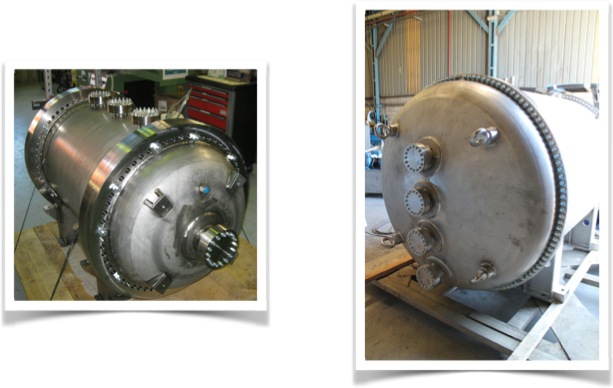
\includegraphics[height=8cm]{img/PV.png}
\caption{The NEW (left) and NEXT-100 (right) PV.} \label{fig:PV}
\end{figure}


\subsubsection*{Objectives of the COORD subproject}

{\bf Construction of the NEW and NEXT-100 pressure vessels (WP1)}

The NEW and NEXT-100 pressure vessels, shown in Figure \ref{fig:PV} were designed to withstand pressures in excess of 20 bar, and to operate with negligible losses at 15 bar. They are built using a 316Ti alloy of low activity ($\sim$0.2 mBq/kg for the thorium series and 
the uranium series, as measured by our screening campaign). The PVs have been payed from CUP funds. Inside the PVs an innder copper shielding (ICS) made of ultra pure copper bars of 6 cm (in the case of NEW) and 12 cm (in the case of NEXT-100) shield the gas volume from the residual radiation emitted by the lead shielding and the PV. The ICS of both systems will be payed using AdG funds. 

The design of the PV was a collaboration between IFIC and LBNL groups. Manufacturing has involved several companies in Spain and has benefited from a CEDETI grant. The remaining activities in the project, which involves engineering personnel from IFIC and UPV is the construction and installation of the ICS for both NEW and NEXT-100. 

